\documentclass[problem]{mcs}

\begin{pcomments}
  \pcomment{CP_coin_flip_sequences}
  \pcomment{second part of PS_coin_flip_sequences}
\end{pcomments}

\pkeywords{
  conditional_probability
  total_probability
  transitive
  intransitive
  infinite_tree
}

%%%%%%%%%%%%%%%%%%%%%%%%%%%%%%%%%%%%%%%%%%%%%%%%%%%%%%%%%%%%%%%%%%%%%
% Problem starts here
%%%%%%%%%%%%%%%%%%%%%%%%%%%%%%%%%%%%%%%%%%%%%%%%%%%%%%%%%%%%%%%%%%%%%

\begin{problem}
Suppose you repeatedly flip a fair coin until you see the sequence
\STR{HTT} or \STR{HHT}.  What is the probability you see the
sequence \STR{HTT} first?

\hint Try to find the probability that \STR{HHT} comes before
\STR{HTT} conditioning on whether you first toss an \STR{H} or a
\STR{T}.  The answer is not $1/2$.

\begin{solution}
We apply the standard tree diagram approach where the $n$th level of
the tree corresponds to the results of the $n$th coin flip.  This tree
is infinite, but we need not be intimidated: the tree has a repeating
structure which allows a simple recursive description.  Then the Law
of Total Probability applied to the recursive tree structure will lead
to some simple equations for the desired probability.

To see how this works, suppose our first toss is \STR{T}.  Since
neither of our patterns starts with \STR{T}, the situation relevant to
our patterns is the same as at the start.  So if we let $A$ be the
tree diagram describing our coin flipping experiment, then the branch
corresponding to flipping \STR{T} goes to a copy of $A$.  This is
illustrated in Figure~\ref{HTTHHT}.

\begin{figure}[h]
  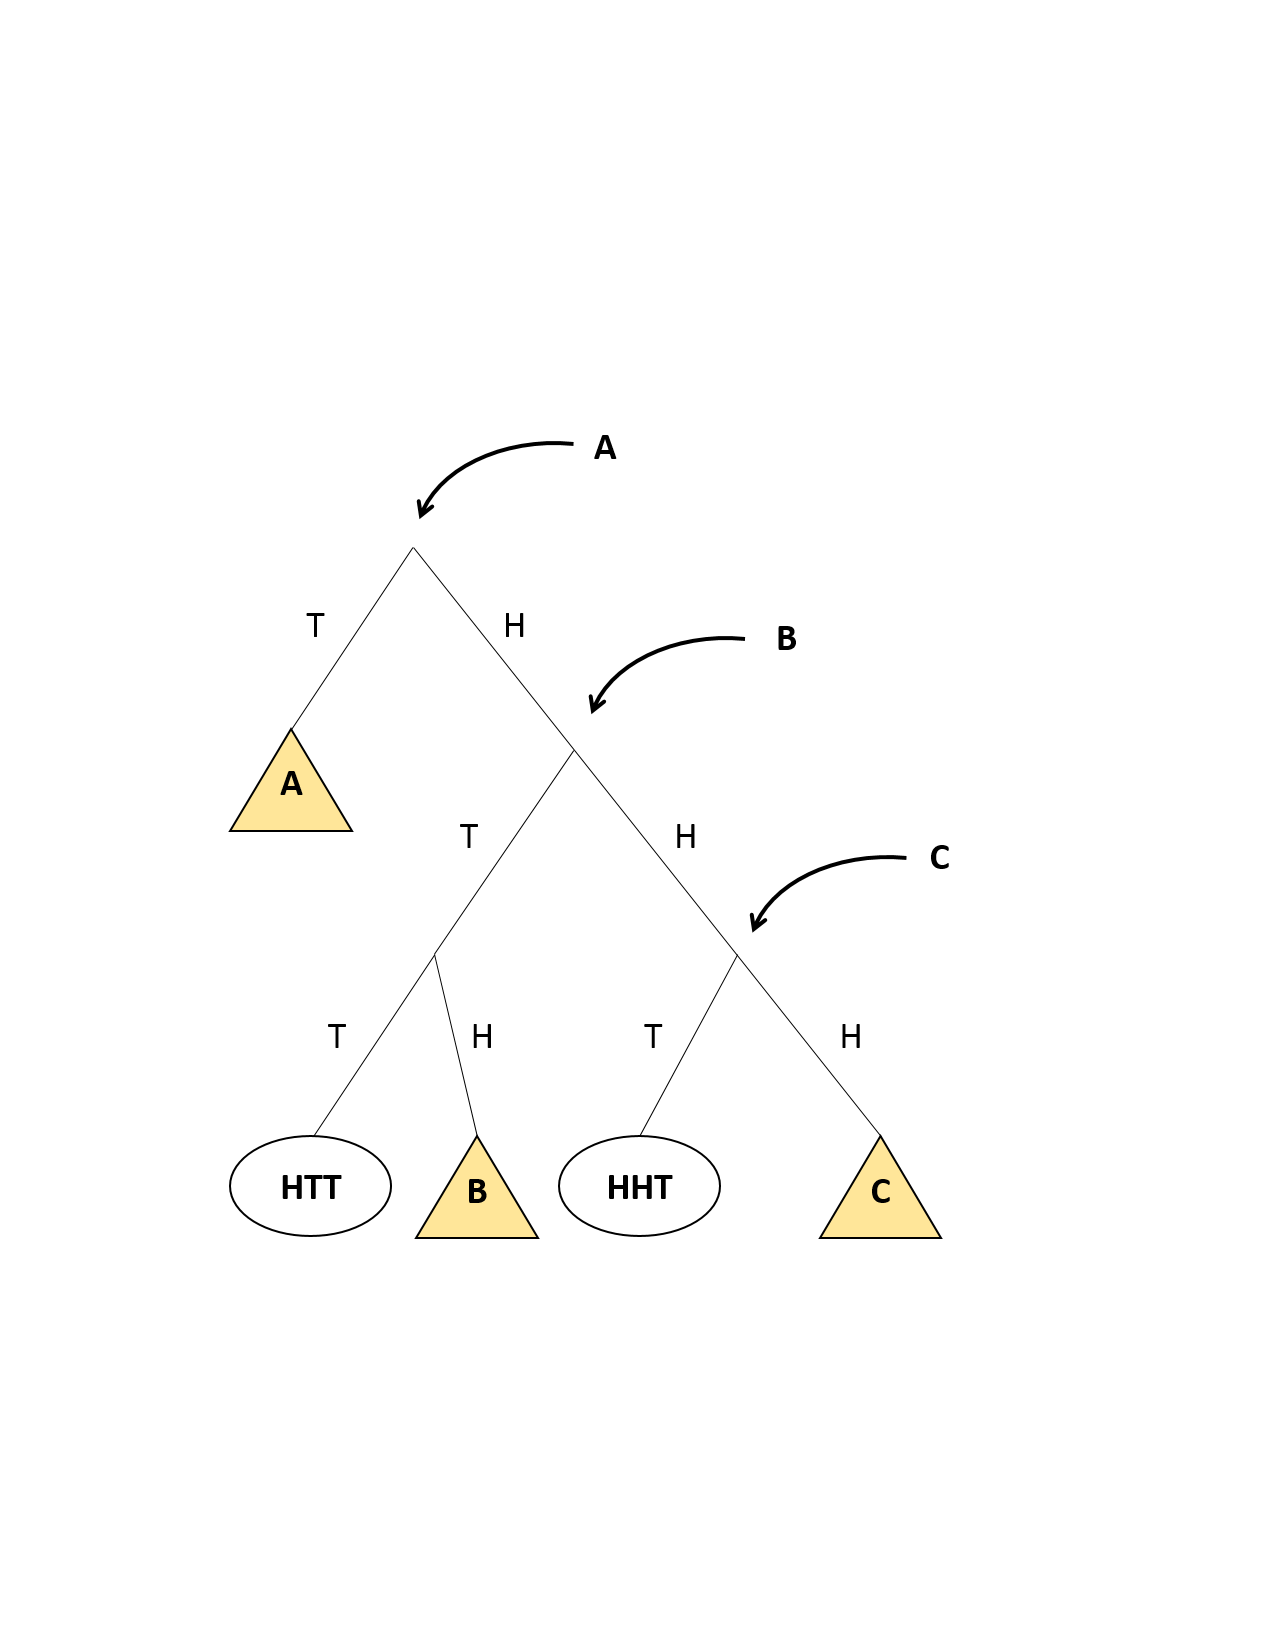
\includegraphics[width=4.5in]{HTT_HHT_race}
  \caption{\STR{HTT} versus \STR{HHT}.}
  \label{HTTHHT}
\end{figure}

If our first flip is \STR{H}, we need to consider different cases
based on the subsequent throws.  So let $B$ be the subtree
corresponding the first flipping \STR{H}, and let $C$ be the subtree
corresponding to the second flip also being \STR{H}.  Now if the third
flip is \STR{T}, then we arrive at the leaf where \STR{HHT} has
occurred first.  On the other hand, if the third flip is \STR{H}, then
the first flip is no longer relevant to the length three patterns we
are considering, and we are at the same point in progressing toward
our patterns as we were after flipping only two \STR{H}'s.  That is,
the \STR{H} branch of subtree $C$ is another copy of $C$.  This is
also illustrated in Figure~\ref{HTTHHT}.  We finish up by observing
that if the first three flips are \STR{HTT}, then we arrive at the
leaf where \STR{HTT} has occurred first, and if the first
three flips are \STR{HTH}, then the situation is the same as if we
first flipped \STR{H}.  So the subtree at after \STR{HTH} is the same
as $B$.

This completes the reasoning which led to the tree diagram illustrated
in Figure~\ref{HTTHHT}.

Now let $E$ be the event that \STR{HTT} appears before \STR{HHT}.  Our
task is to calculate $\pr{E}$.  Since the tree $A$ describes the start
of the coin flipping, we have
\[
\pr{E} = \prcond{E}{A}.
\]

Next, by the Law of Total Probability,
\begin{equation}\label{EAEAT}
\prcond{E}{A} = \prcond{E}{A} \cdot \pr{\STR{T}} + \prcond{E}{B} \cdot \pr{\STR{H}},
\end{equation}
which implies
\begin{equation}\label{EA=EB}
\prcond{E}{A} = \prcond{E}{B}.
\end{equation}

Again by the Law of Total Probability,
\begin{align}
\prcond{E}{B}
    & = \prcond{E}{B\STR{TT}} \cdot \pr{\STR{TT}}
       + \prcond{E}{B\STR{TH}} \cdot \pr{\STR{TH}}
       + \prcond{E}{B\STR{H}} \cdot \pr{\STR{H}}\notag\\
    & = 1 \cdot \frac14 + \prcond{E}{B}\cdot \frac14
            + \prcond{E}{C} \cdot  \frac12,\label{114EB}\\
\prcond{E}{C}
   & = \prcond{E}{C\STR{T}} \cdot \pr{\STR{T}}
       + \prcond{E}{C\STR{H}} \cdot \pr{\STR{H}}\notag\\
   & = 0 \cdot \frac12 +  \prcond{E}{C} \cdot \frac12. \label{012EC}
\end{align}
Now from~\eqref{012EC} we immediately get
\[
\prcond{E}{C} = 0.
\]
Then from~\eqref{114EB},
\begin{align*}
\prcond{E}{B} & = \frac14 + \prcond{E}{B} \cdot \frac14,\\
\prcond{E}{B} & = \frac13,
\end{align*}
and so by~\eqref{EA=EB}
\[
\prcond{E}{A} = \frac13.
\]
That is, \STR{HTT} appears before \STR{HHT} with probability 1/3.

These kind of events have an amazing \idx{intransitivity} property: if
you pick \emph{any} pattern of three flips such as \STR{HTT}, then I
can pick a pattern of three flips such as \STR{HHT} whose odds of
coming up first are better then even.  In particular, even if you
instead picked the ``better'' pattern \STR{HHT}, there is another
pattern I can pick that has a more than even chance of appearing
before \STR{HHT}.\footnote{To learn the simple recipe for picking a
  better pattern and much more about races to reach coin flip patterns
  see
  \href{https://sites.math.washington.edu/~mathcircle/circle/2015-16/second/PenneyAnte.pdf}
       {\emph{Penney Ante: Counterintuitive Probabilities in Coin
           Tossing}, R.S. Nickerson}}



\iffalse
So there are cases where a pattern 1 appears before a pattern 2 with
probability better than one half, and pattern 2 appears before a
pattern 3 with probability better than one half, and pattern 3 also
appears before pattern 1 with probability better than one half.
\fi

So we leave you with an ethical dilemma: is it OK to allow a naive
opponent to first choose whichever pattern of three flips he likes
best, then you choose your own preferred pattern, after which you bet
real money on the coin flip game?
\end{solution}

\end{problem}

%%%%%%%%%%%%%%%%%%%%%%%%%%%%%%%%%%%%%%%%%%%%%%%%%%%%%%%%%%%%%%%%%%%%%
% Problem ends here
%%%%%%%%%%%%%%%%%%%%%%%%%%%%%%%%%%%%%%%%%%%%%%%%%%%%%%%%%%%%%%%%%%%%%

\endinput

\iffalse

Suppose our first flip is \STR{T}.  Since neither of our patterns
starts with \STR{T}, the probability that $A$ will occur from this
point on is still $p$.  That is, $\prcond{A}{\tails} = p$.

Suppose our first flip is \STR{H}.  To find the probability that $A$
will now occur, that is, to find $r \eqdef \prcond{A}{\heads}$, we
consider different cases based on the subsequent throws.

Suppose the next flip is \STR{H}, that is, the first two flipes are
\STR{HH}.  Then neither pattern appears if we continue flipping
\STR{H}, and when we eventually flip a \STR{T}, the pattern
\STR{HHT} will then have appeared first.  So in this case, event $A$
will never occur.  That is $\prcond{A}{\mathtt{HH}} = 0$.

Suppose the first two flipes are \STR{HT}.  If we flip a \STR{T}
again, then we have fliped \STR{HTT}, so event $A$ has occurred.
If we next flip an \STR{H}, then we have fliped \STR{HTH}.  But this
puts us in the same situation we were in after rolling an \STR{H} on
the first flip.  That is, $\prcond{A}{\mathtt{HTH}} = r$.
\fi



Let $E$ be the event that \STR{HTT} appears before \STR{HHT}, and let
$p \eqdef \prob{A}$.

Let $\pr{A}$ be the of seeing \STR{HTT} before \STR{HHT} if
you start at $A$, and define $pr{B}$ and $pr{C}$ similarly.  We are
trying to find $pr{A}$.

%, that is, the probability of seeing \STR{HTT} before \STR{HTT} if
%you start with no prior information.

Then,
\begin{align*}
Pr[A] &  = \frac12 Pr[A] + \frac12 Pr[B]\\
Pr[B] & = \frac14 + \frac14 Pr[B] + \frac14 Pr[C]\\
Pr[C] & = \frac12 Pr[C]
\end{align*}
Solving these equations (starting from the bottom going up), we get
\begin{align*}
            Pr[C] & = 0\\
Pr[B] - 1/4 Pr[B] & = 1/4 + 0\\
            Pr[B] & = 1/3\\
Pr[A] - 1/2 Pr[A] & = 1/2 * 1/3\\
            Pr[A] & = 1/3.
\end{align*}
So \STR{HTT} comes before \STR{HHT} with probability 1/3.
\fi

